\chapter{Result}
\section{Total water storage}
As mentioned in chapter 3, 4 time series (CSR, GFZ, ITSG, JPL) of TWSA from Apr. 2002 to May. 2020 are handled in this work. By using the method in \autoref{sec:Gaussmarkov}, these four time series can be summarized into one time series \autoref{fig:twsa}. It is shown that the TWSA increases in summer and decreases in winter annually.As can be seen in this figure, the TWS remains relative stable. We can also see an positive trend from 2013 to 2017 and a negative trend from 2010 to 2012 and after 2017.   \\
\begin{figure}[htbp]\centering
	\begin{minipage}[t]{0.85\textwidth}
		\centering
		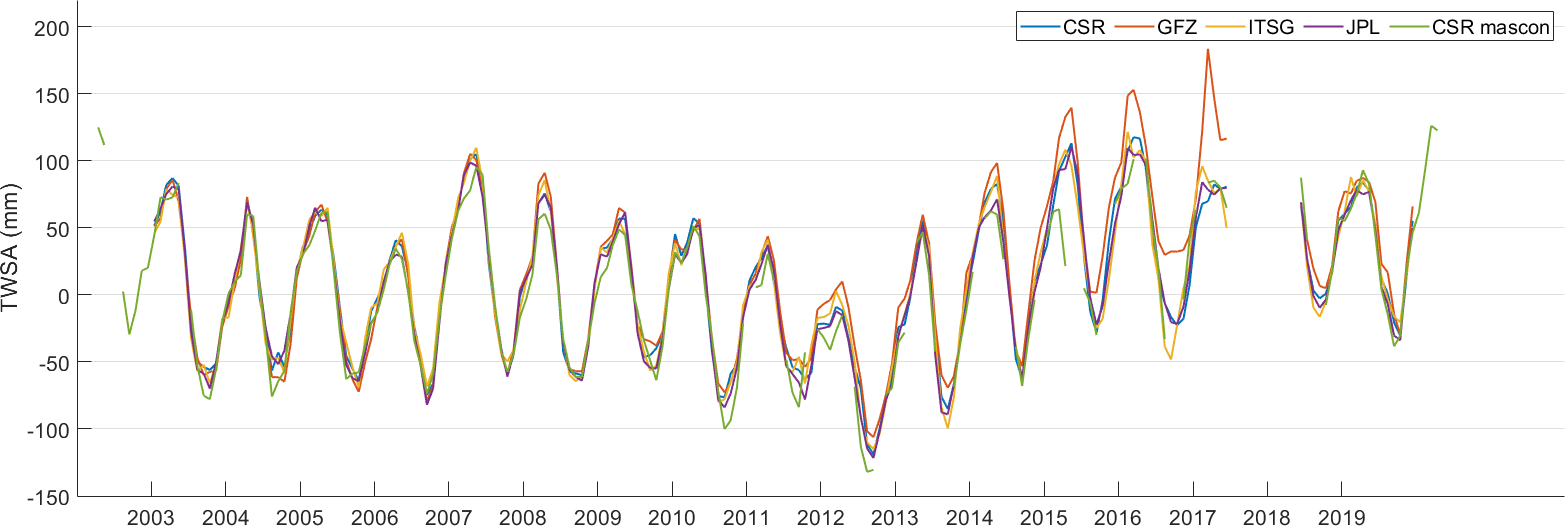
\includegraphics[width=1\textwidth]{TWSAall} % Datei in "bilder/" bei LaTeX: eps, bei PDFLaTeX: jpg (o.ä.) 
	\end{minipage}
	\begin{minipage}[t]{0.85\textwidth}
		\centering
		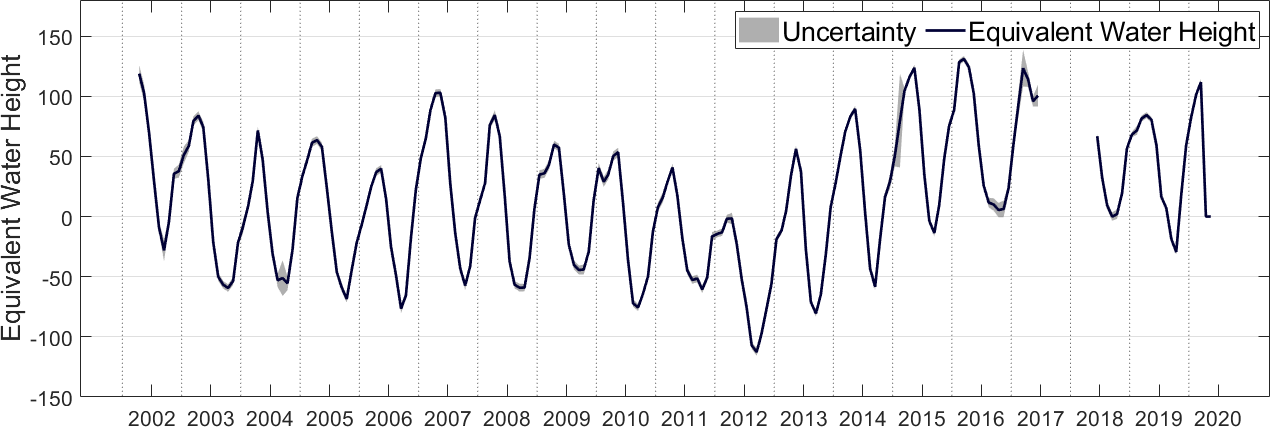
\includegraphics[width=1\textwidth]{EWH} % Datei in "bilder/" bei LaTeX: eps, bei PDFLaTeX: jpg (o.ä.) 
	\end{minipage}
	\caption{TWSA generated from different data centers (top) generate one summarized TWSA time series (bottom) from Jan.2003 to Dec.2019}
	\label{fig:twsa}
\end{figure}\\
By using the methods in \autoref{eq:dsdt} and \autoref{sec:Gaussmarkov} 2 abrupt change in the deviation of TWSA are found. The time of these two points are October of 2012 and November of 2015, which proves the assumption of positive trend above, while the negative trend between 2010 and 2012 can not determined. With this 2 points the whole time series can divide into 3 periods.
\begin{figure}[htbp]\centering
	\begin{minipage}[t]{0.7\textwidth}
		\centering
		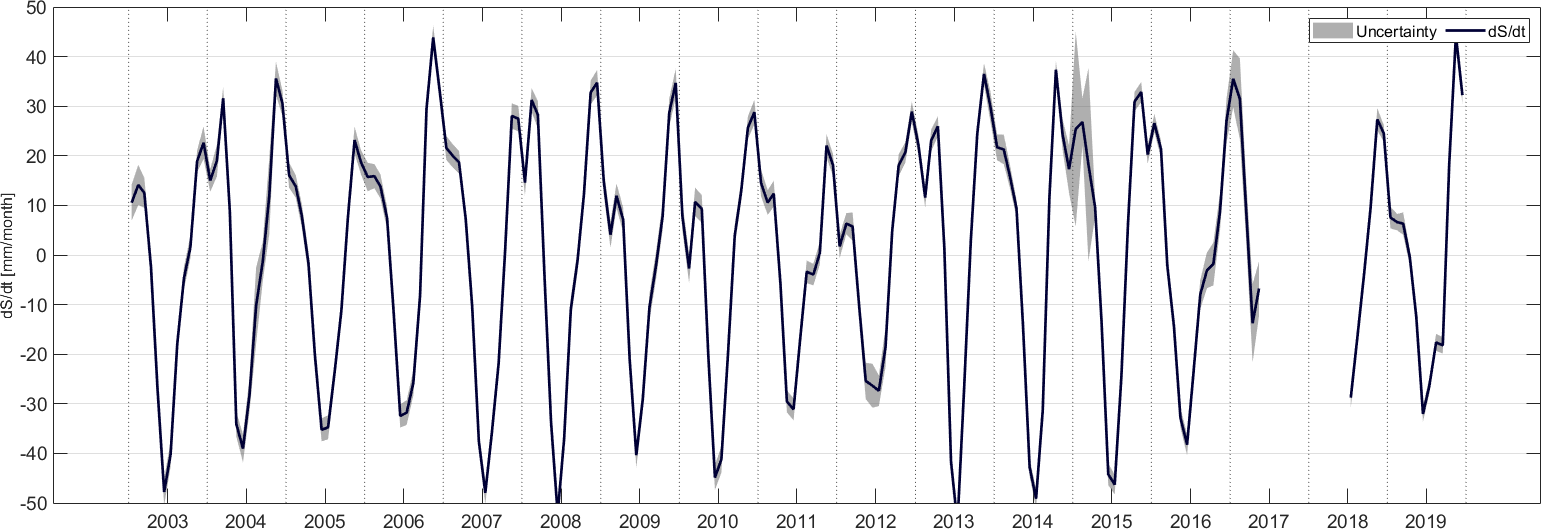
\includegraphics[width=1\textwidth]{dSdt} % Datei in "bilder/" bei LaTeX: eps, bei PDFLaTeX: jpg (o.ä.) 
	\end{minipage}
	\begin{minipage}[t]{0.7\textwidth}
		\centering
		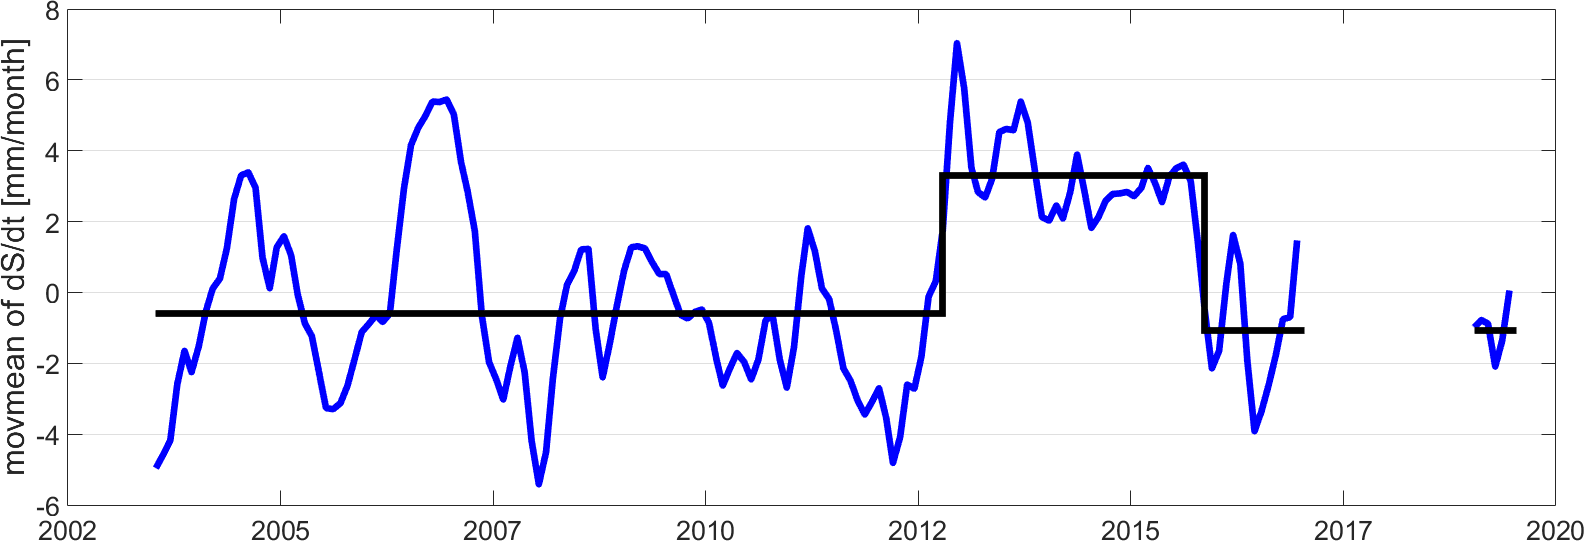
\includegraphics[width=1\textwidth]{dSdtmovmean} % Datei in "bilder/" bei LaTeX: eps, bei PDFLaTeX: jpg (o.ä.) 
	\end{minipage}
	\caption{the derivation of TWSA (top) and the abrupt change in the moving average (bottom)}
	\label{fig:dsdt}
\end{figure}\\
After that, the mean $dS/dt$ along with uncertainty in these 3 periods can be calculated \autoref{fig:dsdtnum}, it is shown that in the first and the third period $dS/dt$ are negative, while in the second period the value is positive. This indicates, that the TWS in the first and the third period were decreasing while the basin has gained water from outside in the second period.  \\
\begin{figure}[htbp]
	\centering
	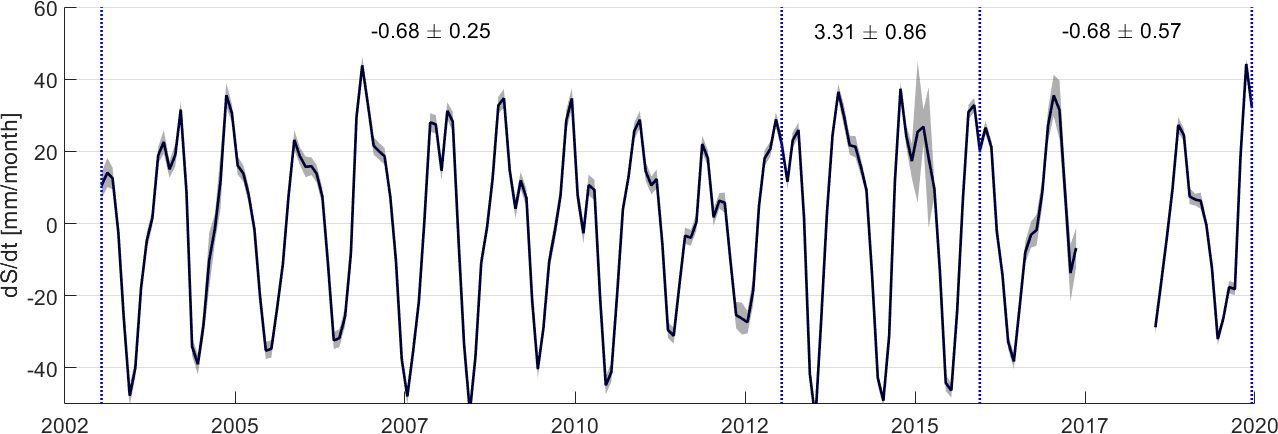
\includegraphics[width=0.7\textwidth]{dSdtwithnum} 
	\caption{mean value with uncertainty of dS/dt and RMSE in 3 periods} 
	\label{fig:dsdtnum}
\end{figure}\\
As mentioned in chapter 2, the Ob river basin contains a big area. Therefore, it's necessary to confirm, that the behavior of total water storage change is similar among the basin. \autoref{fig:twsspatial} provides mean TWS trend in three periods in Ob basin in gridded area. In the first period, the total water storage remained unchanged in east part but had an slight reduce in west. In the second period, the wast north of the basin obtained a large amount water from outside, but in south east not that much. In the third period, the north west and south east suffered water lost. 
\begin{figure}[htbp]\centering
	\begin{minipage}[t]{0.3\textwidth}
		\centering
		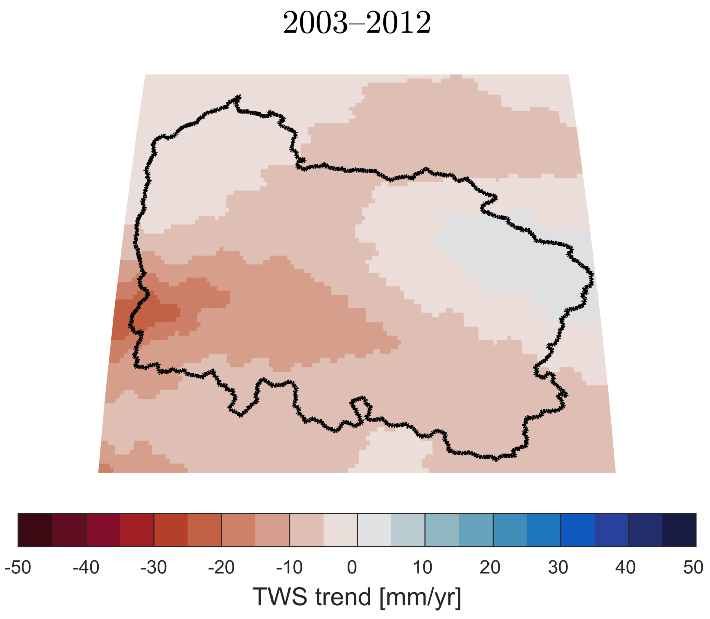
\includegraphics[width=1\textwidth]{trend1} % Datei in "bilder/" bei LaTeX: eps, bei PDFLaTeX: jpg (o.ä.) 
	\end{minipage}
	\begin{minipage}[t]{0.3\textwidth}
		\centering
		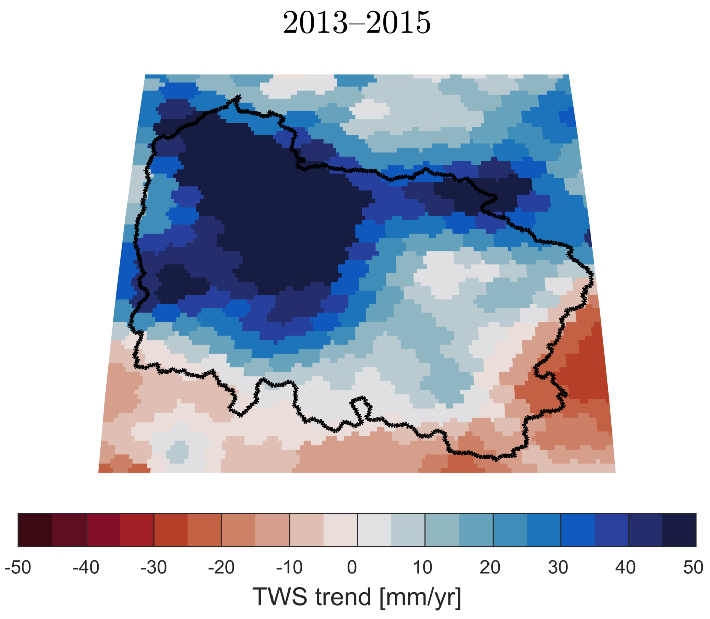
\includegraphics[width=1\textwidth]{trend2} % Datei in "bilder/" bei LaTeX: eps, bei PDFLaTeX: jpg (o.ä.) 
	\end{minipage}
	\begin{minipage}[t]{0.3\textwidth}
		\centering
		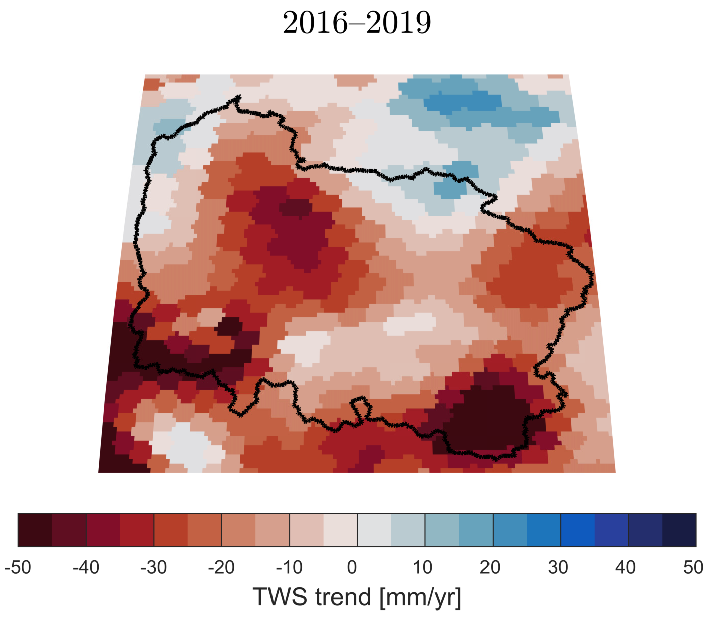
\includegraphics[width=1\textwidth]{trend3} % Datei in "bilder/" bei LaTeX: eps, bei PDFLaTeX: jpg (o.ä.) 
	\end{minipage}
	\caption{spatial TWS change of Ob river basin in each period using mascon CSR RL06 solution}
	\label{fig:twsspatial}
\end{figure}
\section{Precipitation}
It was mentioned in chapter 3 that precipitation data from 9 datasets are processed and one time series with uncertainty can be generated by summarizing them \autoref{fig:prenum} just as before. The uncertainty are calculated using methods mentioned in \autoref{sec:Gaussmarkov}.
\begin{figure}[htbp]\centering
	\begin{minipage}[t]{0.9\textwidth}
		\centering
		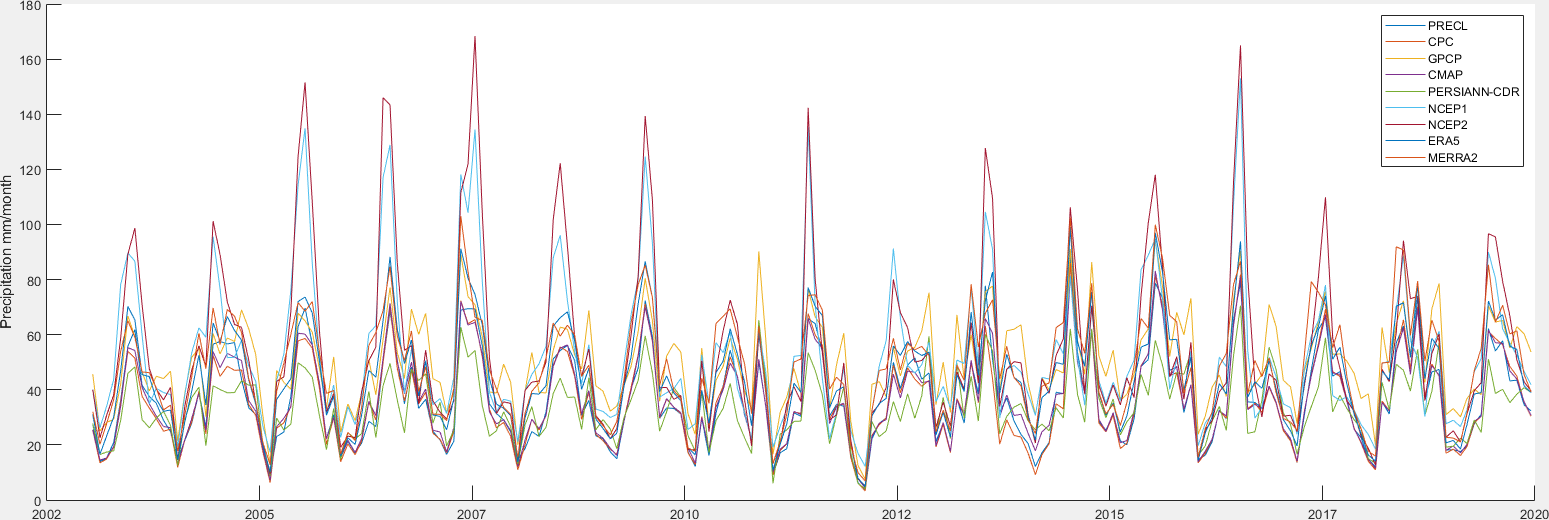
\includegraphics[width=0.9\textwidth]{precenter} % Datei in "bilder/" bei LaTeX: eps, bei PDFLaTeX: jpg (o.ä.) 
	\end{minipage}
	\begin{minipage}[t]{0.9\textwidth}
		\centering
		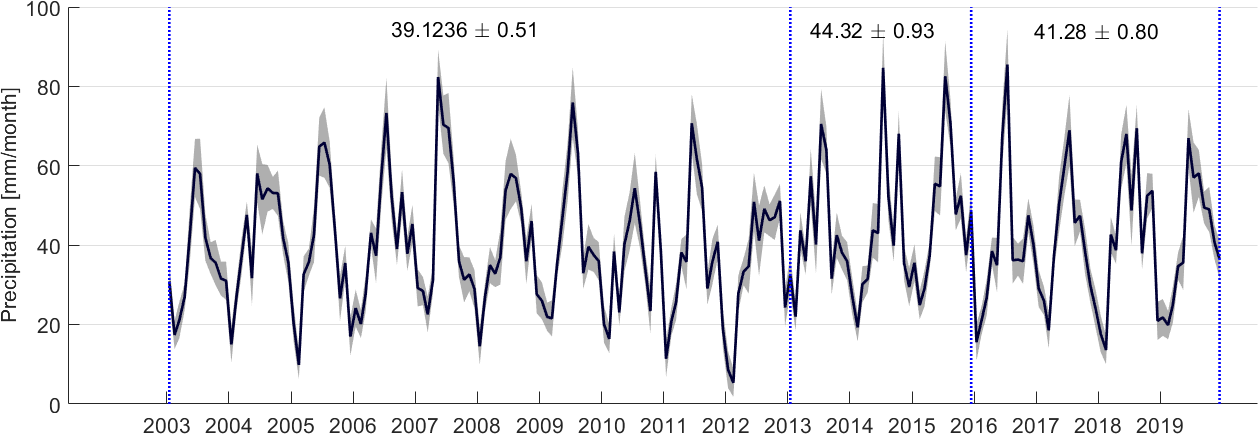
\includegraphics[width=0.9\textwidth]{precipitationwithnumber} % Datei in "bilder/" bei LaTeX: eps, bei PDFLaTeX: jpg (o.ä.) 
	\end{minipage}
	\caption{all precipitation datasets (top) are summarized into one time series, the mean precipitation with RMSE in 3 periods are calculated (bottom)}
	\label{fig:prenum}
\end{figure}
\begin{figure}[htbp]\centering
	\centering
	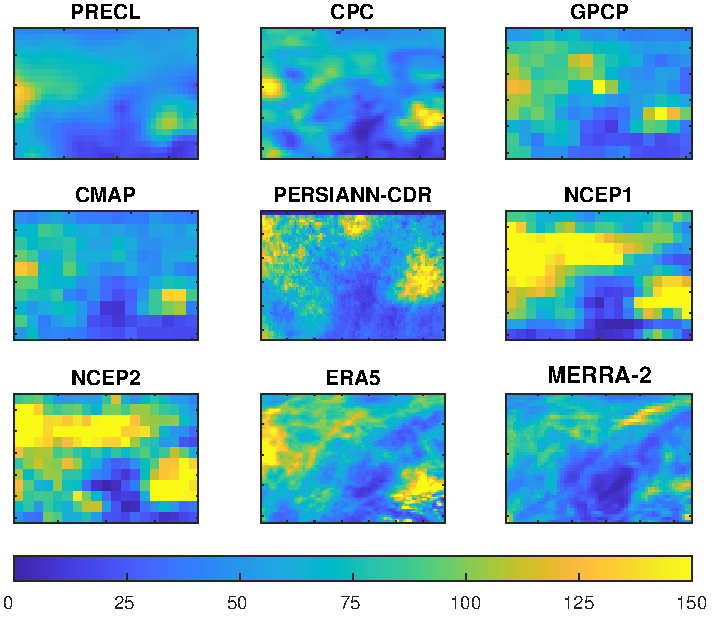
\includegraphics[width=0.45\textwidth]{Pre_spatial_June2003} % Datei in "bilder/" bei LaTeX: eps, bei PDFLaTeX: jpg (o.ä.) 
	\caption{spatial change of precipitation in Ob river basin using different datasets in June of 2003} 
	\label{fig:spatialpre}
\end{figure}\\\\
By using the same methods for $dS/dt$, the precipitation are considered into 3 periods, the mean value and uncertainties show that in the second periods the amount of precipitation in this area is $5.2\ut{mm/month}$ bigger than the first period. The precipitation in the third period, however, is less than the second period but still more than the first period.\\\\
The spatial information of precipitation from different datasets is also presented \autoref{fig:spatialpre}. The data in June of 2003 are taken since the precipitation reaches the summit normally in summer. AS we can see, in spite of the different spatial resolution of different datasets it can be detected that the major part of the precipitation took place in west north and east north. 
% all precipitation in one 
\section{Evapotranspiration}
Like precipitation, the summarized evapotranspiration is presented temporally and the time series is split into 3 periods. The mean value along with uncertainty are also calculated. From \autoref{fig:etnum} we can see that the evapotranspiration reaches the summit in summer but nearly disappear in the winter. The results of evapotranspiration is similar to what we see in precipitation: it increases in the second period by $1.54 \ut{mm/month}$ and decreases after Dec. 2015 and it didn't go back to the original level in the first period like precipitation. It should also be noted that evapotranspiration has not increased that much in the second period as in precipitation, which follows the rules of water cycle.
\begin{figure}[htbp]\centering
	\begin{minipage}[t]{0.9\textwidth}
		\centering
		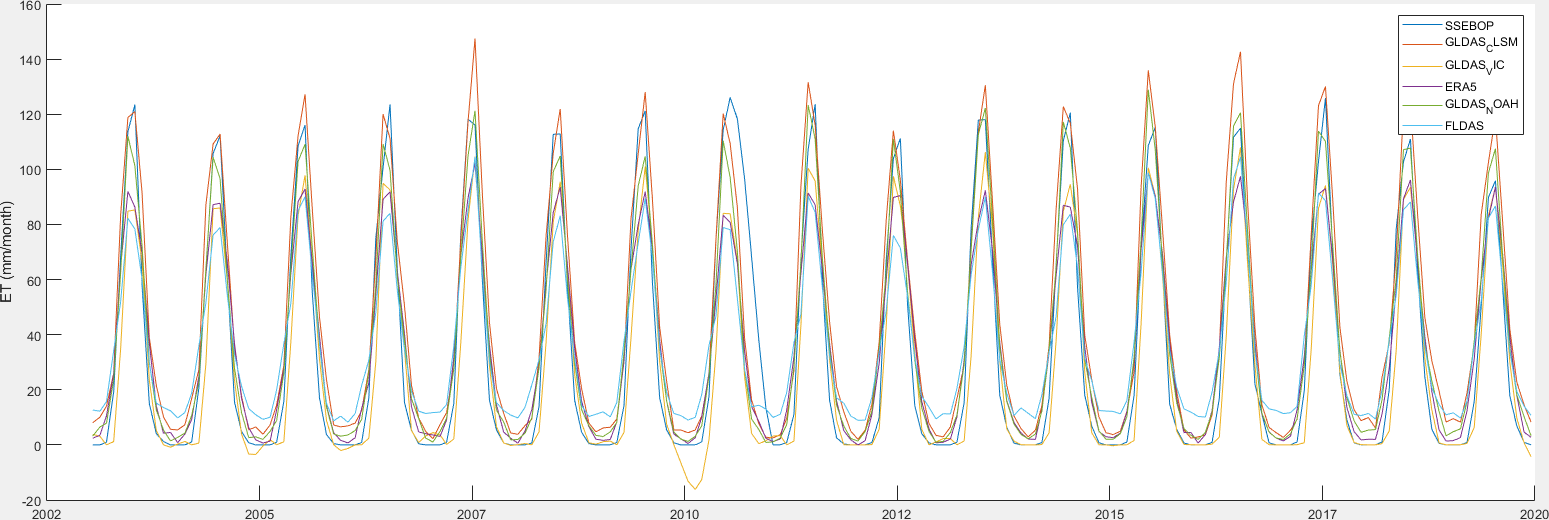
\includegraphics[width=0.9\textwidth]{etcenter} % Datei in "bilder/" bei LaTeX: eps, bei PDFLaTeX: jpg (o.ä.) 
	\end{minipage}
	\begin{minipage}[t]{0.9\textwidth}
		\centering
		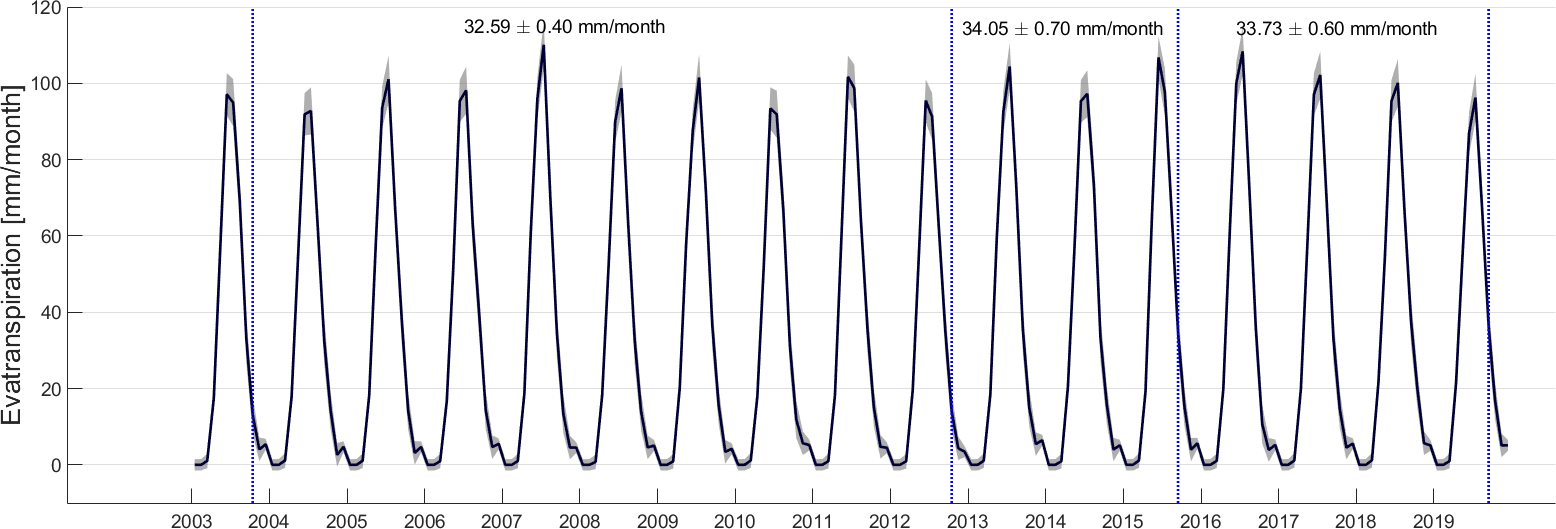
\includegraphics[width=0.9\textwidth]{etall} % Datei in "bilder/" bei LaTeX: eps, bei PDFLaTeX: jpg (o.ä.) 
	\end{minipage}
	\caption{all evapotranspiration datasets (top) are summarized into one time series, the mean precipitation with uncertainty in 3 periods are calculated (bottom)}
	\label{fig:etnum}
\end{figure}\\\\
The spatial information of evapotranspiration is concluded in \autoref{fig:spatialet}. Same as precipitation, the data from June of 2003 are used for this figure. By comparing different datasets we can find that the evapotranspiration occurs stronger in the east part of the basin.
\begin{figure}[htbp]\centering
	\centering
	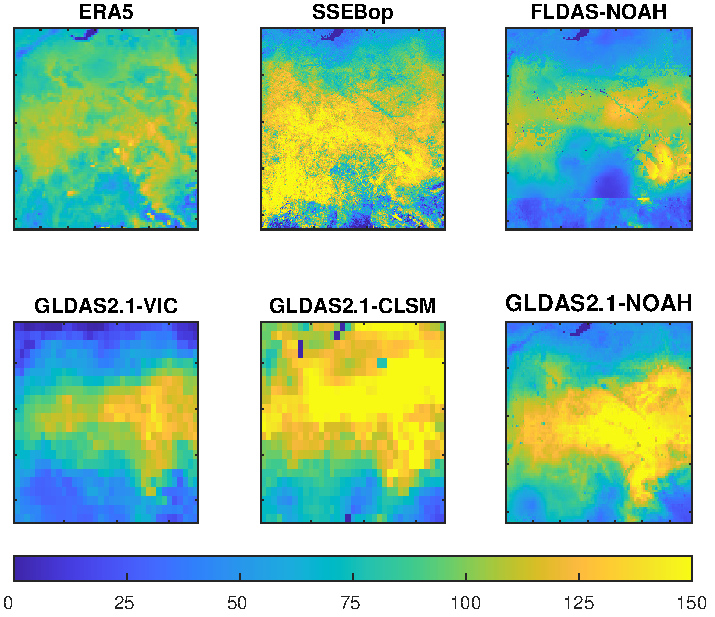
\includegraphics[width=0.45\textwidth]{ET_spatial_June2003} % Datei in "bilder/" bei LaTeX: eps, bei PDFLaTeX: jpg (o.ä.) 
	\caption{spatial change of evapotranspiration in Ob river basin using different datasets in June of 2003} 
	\label{fig:spatialet}
\end{figure}
\clearpage
\section{Runoff}
\subsection{Runoff from global datasets}
Like precipitation and evapotranspiration, Runoff data estimated from several models are provided and meanwhile the in-situ data till end of 2010 is available \autoref{fig:rcenter}. It can been seen that the differences between models and in-situ data are not small.  By calculating RMSE for these models the quality of them can be estimated. \autoref{tab:runofferror} provides the RMSE for all these datasets, the smallest RMSE is already bigger than 8\ut{mm/month}, which is hardly to trust for further analyze. 
\begin{figure}[htbp]\centering
	\centering
	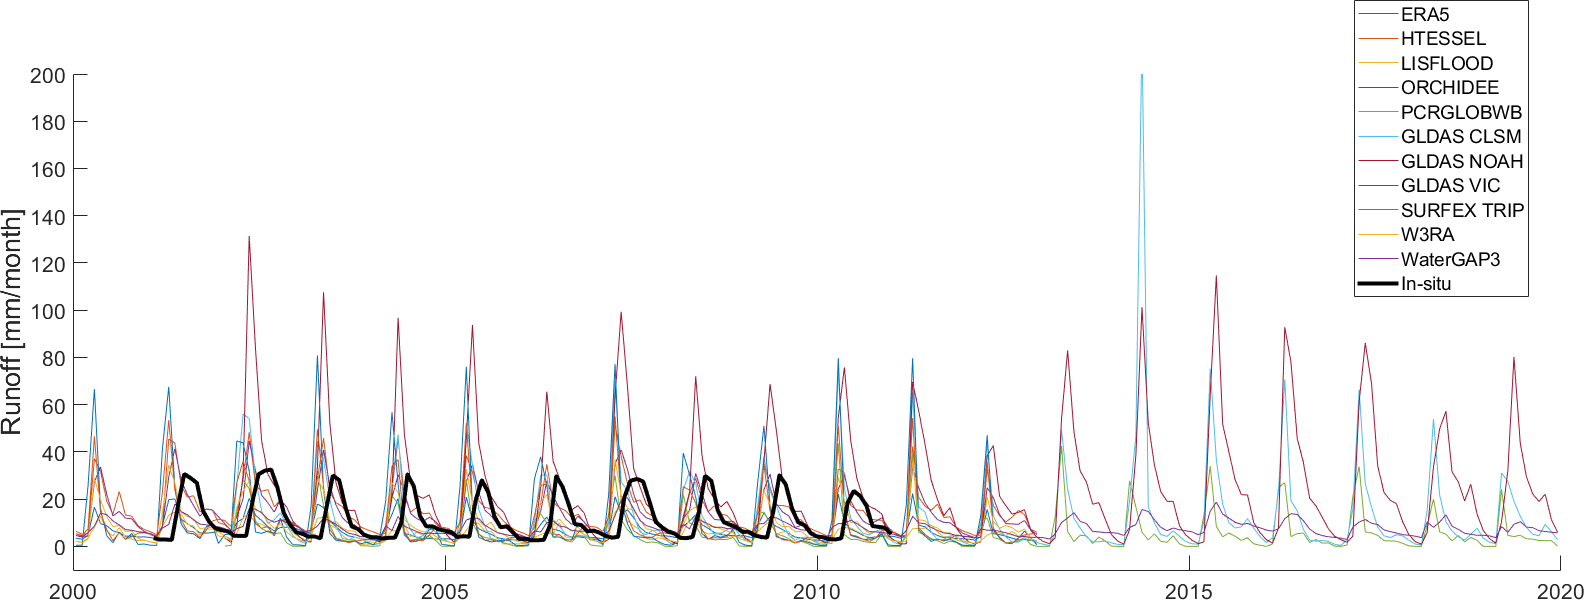
\includegraphics[width=0.9\textwidth]{runoffcenter} % Datei in "bilder/" bei LaTeX: eps, bei PDFLaTeX: jpg (o.ä.) 
	\caption{Runoff datasets, the black bold time series is the in-situ runoff} 
	\label{fig:rcenter}
\end{figure}
\begin{table}[htbp]\label{tab:rmse} \centering
	\begin{tabular}{|l|c|}
		\hline
		Datacenter  & RMSE (mm/month) \\ \hline
		ERA5        & 8.18  \\ \hline
		HTESSEL     & 10.40 \\ \hline
		LISFLOOD    & 11.92 \\ \hline
		ORCHIDEE    & 10.24 \\ \hline
		PCRGLOBWB   & 9.48  \\ \hline
		GLDAS CLSM  & 13.68 \\ \hline
		GLDAS NOAH  & 17.01 \\ \hline
		GLDAS VIC   & 25.95 \\ \hline
		SURFEX-TRIP & 22.05 \\ \hline
		W3RA        & 16.47 \\ \hline
		WaterGAP3   & 11.03 \\ \hline
	\end{tabular}
	\caption{RMSE for runoff datacenters}
	\label{tab:runofferror}
\end{table}\\
Then, if we take the CDF of the difference from those models and in-situ data and set 10\% of mean in-situ runoff as quantile \autoref{fig:rcdf} , it is shown that none of these datasets has achieved the standard (90\%). Therefor, the runoff would be estimated using satellite altimetry. 
\begin{figure}[htbp]
	\centering
	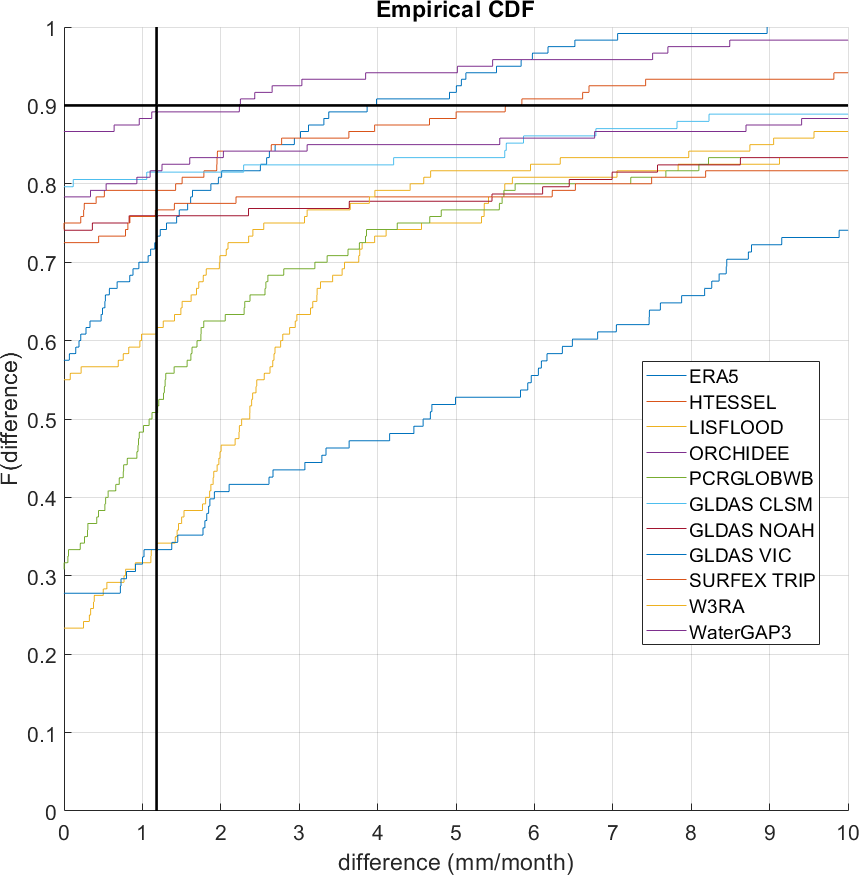
\includegraphics[width=0.6\textwidth]{rcdf} % Datei in "bilder/" bei LaTeX: eps, bei PDFLaTeX: jpg (o.ä.) 
	\caption{CDF of differences} 
	\label{fig:rcdf}
\end{figure}\\
\subsection{Estimating runoff using quantile function and satellite altimetry}
 The methods for runoff estimating is introduced in \autoref{sec:runoff}, \autoref{fig:waterlevel} presents water level time series from Envisat, SARAL and Sentinel. For each mission 2 virtual stations are chosen. In order to get an accurate runoff, water lever from virtual station closer to Salekhard station are used to generated the final runoff. After combining all 3 time series from different space mission, an runoff time series from Jan. 2001 to Dec. 2019 is obtained \autoref{fig:runoff} (top, blue line). Noted that except the gap between Envisat and SARAL, other monthly gaps exists too, these gaps are filled with interpolation \autoref{fig:runoff} (top, red line). \\\\
 Then, as the precipitatin and evapotranspiration, the runoff time series is also divided into 3 periods \autoref{fig:runoff} (bottom) and RMSE is calculated from the method \autoref{sec:waterlevel}. It shows that the runoff in the first periods and in the second periods changes not much, but in the third periods the runoff has increased by about 2 mm/month. However, it was found that the runoff are extremely high in 2 months in summer of 2016, since this unusual peak are not found in the water level time series, these 2 months would be ignored. \ref{fig:rnum2} \\\\
 \begin{figure}[htbp]
 	\centering
 	\begin{minipage}[t]{0.7\textwidth}
 		\centering
 		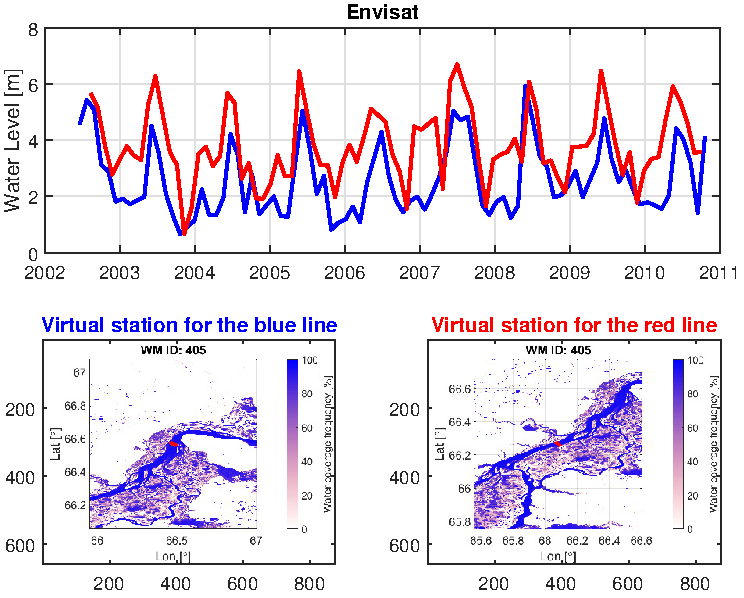
\includegraphics[width=0.8\textwidth]{Envisat_Ob} % Datei in "bilder/" bei LaTeX: eps, bei PDFLaTeX: jpg (o.ä.) 
 	\end{minipage}
 	\begin{minipage}[t]{0.7\textwidth}
 		\centering
 		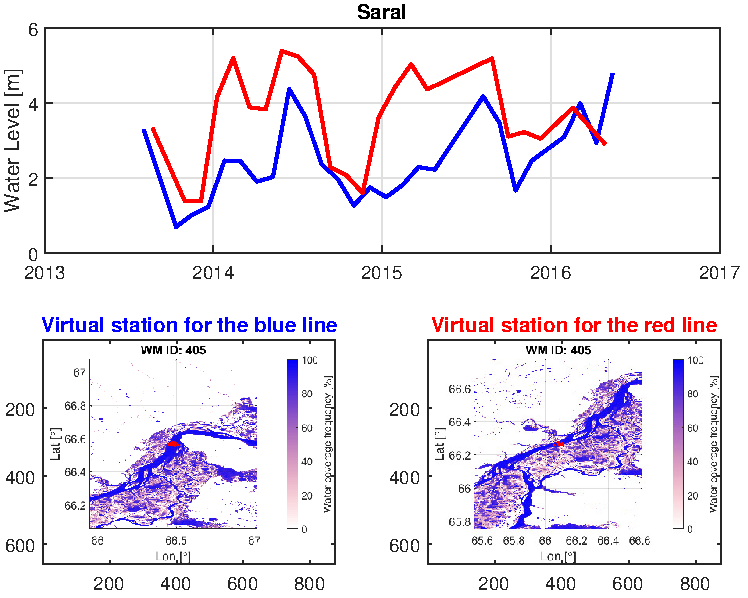
\includegraphics[width=0.8\textwidth]{Saral_Ob} % Datei in "bilder/" bei LaTeX: eps, bei PDFLaTeX: jpg (o.ä.) 
 	\end{minipage}
 \begin{minipage}[t]{0.7\textwidth}
 	\centering
 	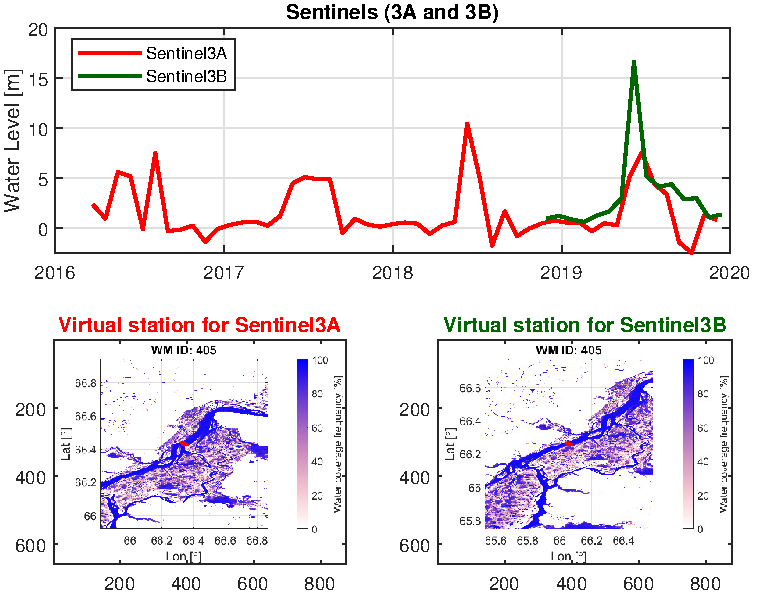
\includegraphics[width=0.8\textwidth]{Sentinels_Ob} % Datei in "bilder/" bei LaTeX: eps, bei PDFLaTeX: jpg (o.ä.) 
 \end{minipage}
 \caption{water level time series and the location of virtual station for different space mission}
 \label{fig:waterlevel}
 \end{figure}
\begin{figure}[htbp]
	\centering
	\begin{minipage}[t]{0.9\textwidth}
		\centering
		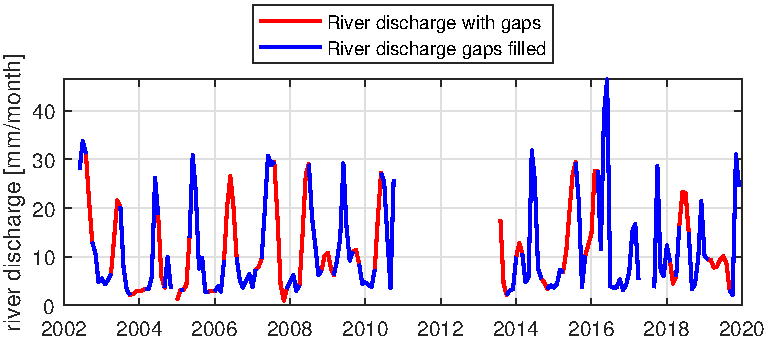
\includegraphics[width=1\textwidth]{Dis_Ob} % Datei in "bilder/" bei LaTeX: eps, bei PDFLaTeX: jpg (o.ä.) 
	\end{minipage}
	\begin{minipage}[t]{0.9\textwidth}
		\centering
		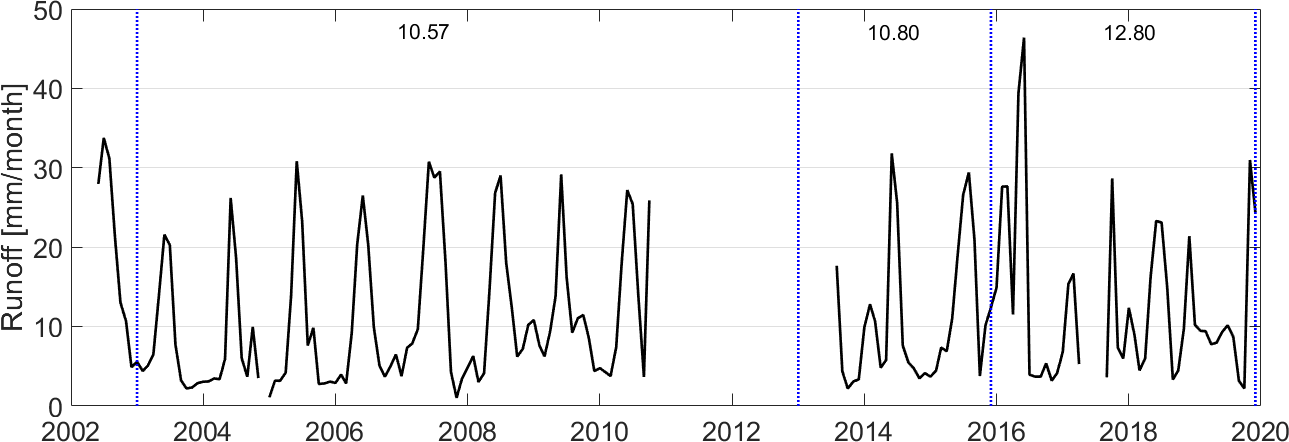
\includegraphics[width=1\textwidth]{runnumber} % Datei in "bilder/" bei LaTeX: eps, bei PDFLaTeX: jpg (o.ä.) 
	\end{minipage}
	\caption{runoff timeseries calculated from water level (top) and the mean value in 3 periods, the red points are unusually high and to be ignored(bottom)}
	\label{fig:runoff}
\end{figure}
\begin{figure}[htbp]
	\centering
		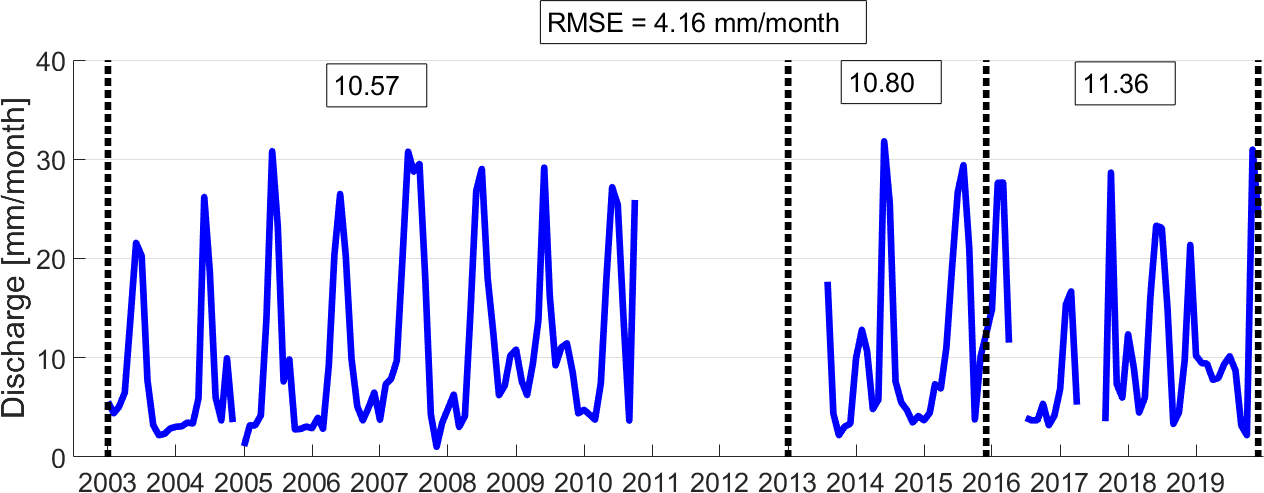
\includegraphics[width=0.9\textwidth]{runoffnumber1} % Datei in "bilder/" bei LaTeX: eps, bei PDFLaTeX: jpg (o.ä.) 
	\caption{runoff time series and mean value in 3 periods after 2 unusual months are ignored} 
	\label{fig:rnum2}
\end{figure}\\
\clearpage
\section{Discussion about the quality}
In order to eliminate the bias between different component, we take the first period as the baseline. Relative dS/dt, precipitaion, evapotranspiration and runoff numbers of other 2 period are obtained related to that. \\\\
In any case, the equation of terrestrial water balance \autoref{equa:waterbalence} has to be a true statement, which means the result of $P-dS/dt-ET-R$ with uncertainties should be 0. Substituing the results of both periods into this formula can get $-0.57 \pm 1.63$ mm/month for the second period, and $0.29 \pm 1.37$ mm/month for the third period, which can be acceptable. 
\begin{table}[htbp]\centering
	\begin{tabular}{|l|c|c|c|}
		\hline
		Period &  2003 to 2012 & 2013 to 2015 & 2016 to 2019  \\ \hline
		$dS/dt$ \ut{(mm/month)}         & $-0.68 \pm 0.25$     & $3.31 \pm 0.86$        & $-0.80 \pm 0.57$        \\ \hline
		$P$     \ut{(mm/month)}        & $39.12 \pm 0.35$      & $44.32 \pm 0.64$       &$41.28 \pm 0.55$        \\ \hline
		$ET$    \ut{(mm/month)}          & $32.59 \pm 0.21$       & $34.13 \pm 0.38$       & $33.78 \pm 0.33$        \\ \hline
		$R$     \ut{(mm/month)}                     & $10.57  \pm 0.51$      & $10.80 \pm 0.94 $     & $11.36 \pm 0.81 $      \\ \hline
		\multicolumn{4}{|l|}{Related to the first period}                                         \\ \hline
		$dS/dt$ \ut{(mm/month)}          &        -     & $4.00 \pm 0.89$        & $-0.11 \pm 0.62$        \\ \hline
		$P$     \ut{(mm/month)}              &       -      & $5.20 \pm 0.72$        & $2.15 \pm 0.65$         \\ \hline
		$ET$    \ut{(mm/month)}          &    -         & $1.53 \pm 0.43$        & $1.19 \pm 0.38 $        \\ \hline
		$R$     \ut{(mm/month)}                   &       -      & $0.23 \pm 1.07 $       & $0.79 \pm 0.96   $      \\ \hline
		$P - dS/dt - ET - R$ \ut{(mm/month)}&       -      & $-0.57 \pm 1.63$       & $0.29 \pm 1.37 $    \\ \hline 
	\end{tabular}
	\caption{mean value of all water cycle component in 3 periods with uncertainties}
\end{table}